\begin{center}
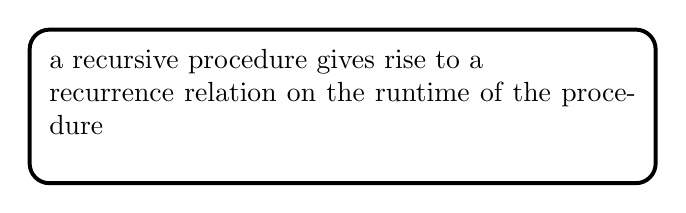
\begin{tikzpicture}

\draw (4.0, 1.0)
  node[draw, line width=0.05cm, , color=black,
       rounded corners=0.25cm, inner sep=0.25cm] {

\begin{minipage}[t][1.45cm]{7.45cm}
\mbox{}

\end{minipage}

};
\draw (4.0, 1.0) node[color=black,
 inner sep=0.25cm] {
 
\begin{minipage}[t][1.45cm]{7.45cm}
a recursive procedure gives rise to a \\ recurrence relation on the runtime of the procedure
\end{minipage}

};
\end{tikzpicture}

\end{center}

